\documentclass[tikz,border=8pt]{standalone}
\begin{document}
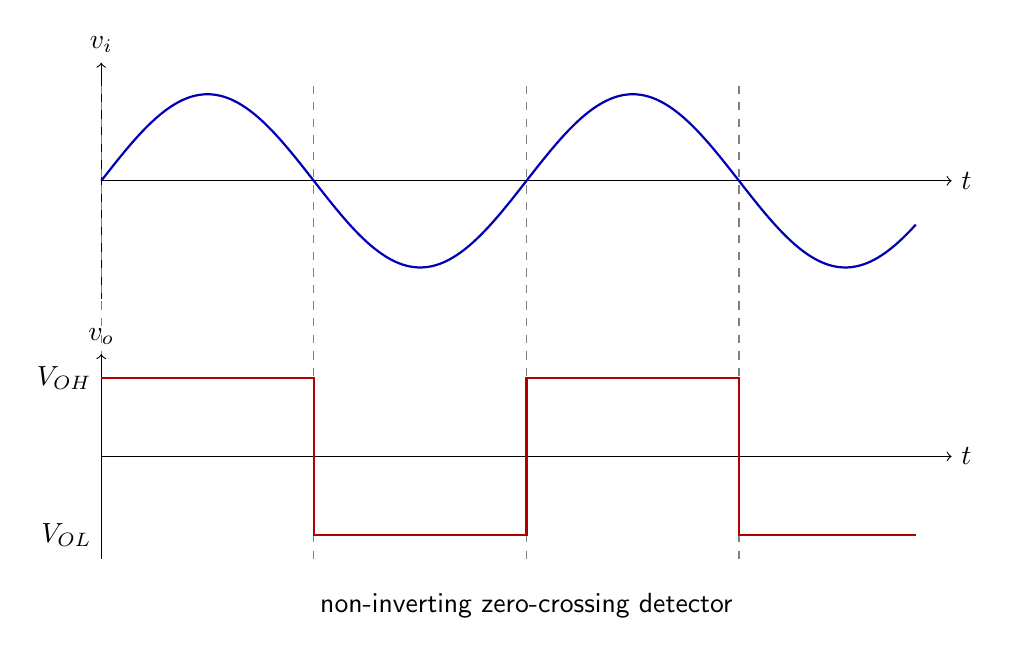
\begin{tikzpicture}[font=\sffamily,x=.9cm,y=1cm]
\draw[->] (0,0)--(12,0) node[right]{$t$};
\draw[->] (0,-1.5)--(0,1.5) node[above]{$v_i$};
\draw[blue!70!black,thick,domain=0:11.5,samples=400] plot (\x,{1.1*sin(60*\x)});
\foreach \x in {0,3,6,9}{\draw[dashed,gray] (\x,-4.8)--(\x,1.2);}
\draw[->] (0,-3.5)--(12,-3.5) node[right]{$t$};
\draw[->] (0,-4.8)--(0,-2.2) node[above]{$v_o$};
\draw[red!70!black,thick] (0,-2.5)--(3,-2.5)--(3,-4.5)--(6,-4.5)--(6,-2.5)--(9,-2.5)--(9,-4.5)--(11.5,-4.5);
\node[left] at (0,-2.5) {$V_{OH}$};
\node[left] at (0,-4.5) {$V_{OL}$};
\node at (6,-5.4) {non-inverting zero-crossing detector};
\end{tikzpicture}
\end{document}
